\documentclass[journal=jacsat,manuscript=article]{achemso}
\usepackage[version=3]{mhchem}
\usepackage{amsmath}
\newcommand*\mycommand[1]{\texttt{\emph{#1}}}
\author{Andrew N. Other}
\altaffiliation{A shared footnote}
\author{Fred T. Secondauthor}
\altaffiliation{Current address: Some other place, Germany}
\author{I. Ken Groupleader}
\affiliation{Department of Chemistry, Unknown University, Unknown Town}
\alsoaffiliation{Department of Chemistry, Second University, Nearby Town}
\altaffiliation{A shared footnote}
\email{i.k.groupleader@unknown.uu}
\phone{+123 (0)123 4445556}
\fax{+123 (0)123 4445557}
\author{Susanne K. Laborator}
\affiliation{Lead Discovery, BigPharma, Big Town, USA}
\email{s.k.laborator@bigpharma.co}
\author{Kay T. Finally}
\affiliation{Department of Chemistry, Unknown University, Unknown Town}
\alsoaffiliation{Department of Chemistry, Second University, Nearby Town}

\abbreviations{IR,NMR,UV}

\keywords{American Chemical Society, \LaTeX}

\title[An \textsf{achemso} demo]{A demonstration of the \textsf{achemso}
\LaTeX~class\footnote{A footnote for the title}}
\makeatletter
\ifxetex
  \usepackage[setpagesize=false, % page size defined by xetex
              unicode=false, % unicode breaks when used with xetex
              xetex]{hyperref}
\else
  \usepackage[unicode=true]{hyperref}
\fi
\hypersetup{breaklinks=true,
            bookmarks=true,
            pdfauthor={},
            pdftitle={},
            colorlinks=true,
            urlcolor=blue,
            linkcolor=magenta,
            pdfborder={0 0 0}}
\urlstyle{same}  % don't use monospace font for urls
\begin{document}
\begin{abstract}
This is an example document for the \textsf{achemso} documentclass,
intended for submissions to the American Chemical Society for
publication. The class is based on the standard \LaTeXe~\textsf{report}
file, and does not seek to reproduce the appearanceof a published paper.

This is an abstract for the \textsf{achemso} document class
demonstration document. An abstract is only allowed for certain
manuscript types. The selection of \texttt{journal} and
\texttt{manuscript} will determine if an abstract is valid. If not, the
class will issue an appropriate error.This is the abstract.
\end{abstract}
\begin{tocentry}
Some journals require a graphical entry for the Table of Contents.
This should be laid out ``print ready'' so that the sizing of the
text is correct.

Inside the \texttt{tocentry} environment, the font used is Helvetica
8\,pt, as required by \emph{Journal of the American Chemical
Society}.

The surrounding frame is 9\,cm by 3.5\,cm, which is the maximum
permitted for  \emph{Journal of the American Chemical Society}
graphical table of content entries. The box will not resize if the
content is too big: instead it will overflow the edge of the box.

This box and the associated title will always be printed on a
separate page at the end of the document.
\end{tocentry}

\section{Introduction}\label{introduction}

This is a paragraph of text to fill the introduction of the
demonstration file. The demonstration file attempts to show the
modifications of the standard \LaTeX~macros that are implemented by the
\textsf{achemso} class. These are mainly concerned with content, as
opposed to appearance.

\section{Results and discussion}\label{results-and-discussion}

\subsection{Outline}\label{outline}

The document layout should follow the style of the journal concerned.
Where appropriate, sections and subsections should be added in the
normal way. If the class options are set correctly, warnings will be
given if these should not be present.

\subsection{References}\label{references}

The class makes various changes to the way that references are handled.
The class loads \textsf{natbib}, and also the appropriate bibliography
style. References can be made using the normal method; the citation
should be placed before any punctuation, as the class will move it if
using a superscript citation style\textsuperscript{1}. The use of
\textsf{natbib} allows the use of the various citation commands of that
package have shown something. Long lists of authors will be
automatically truncated in most article formats, but not in
supplementary information or reviews. If you encounter problems with the
citation macros, please check that your copy of \textsf{natbib} is up to
date. The demonstration database file \texttt{achemso-demo.bib} shows
how to complete entries correctly. Notice that ``\latin{et al.}'' is
auto-formatted using the \texttt{\textbackslash latin} command.

Multiple citations to be combined into a list can be given as a single
citation. This uses the \textsf{mciteplus} package. Citations other than
the first of the list should be indicated with a star.

The class also handles notes to be added to the bibliography. These
should be given in place in the document. As with citations, the text
should be placed before punctuation. A note is also generated if a
citation has an optional note. This assumes that the whole work has
already been cited: odd numbering will result if this is not the case .

\subsection{Floats}\label{floats}

New float types are automatically set up by the class file. The means
graphics are included as follows (Scheme \ref{sch:example}). As
illustrated, the float is ``here'' if possible.

\begin{scheme}
  Your scheme graphic would go here: \texttt{.eps} format\\
  for \LaTeX\, or \texttt{.pdf} (or \texttt{.png}) for pdf\LaTeX\\
  \textsc{ChemDraw} files are best saved as \texttt{.eps} files:\\
  these can be scaled without loss of quality, and can be\\
  converted to \texttt{.pdf} files easily using \texttt{eps2pdf}.\\
  %\includegraphics{graphic}
  \caption{An example scheme}
  \label{sch:example}
\end{scheme}

\begin{figure}[htbp]
\centering
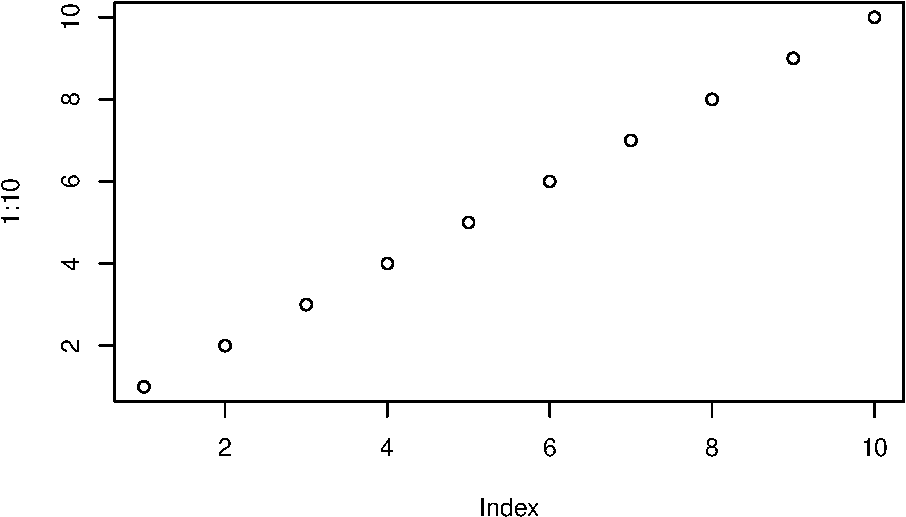
\includegraphics{Untitled_files/figure-latex/unnamed-chunk-1-1.pdf}
\caption{test}
\end{figure}

\begin{figure}
  As well as the standard float types \texttt{table}\\
  and \texttt{figure}, the class also recognises\\
  \texttt{scheme}, \texttt{chart} and \texttt{graph}.
  \caption{An example figure}
  \label{fgr:example}
\end{figure}

Charts, figures and schemes do not necessarily have to be labelled or
captioned. However, tables should always have a title. It is possible to
include a number and label for a graphic without any title, using an
empty argument to the \texttt{\textbackslash caption} macro.

The use of the different floating environments is not required, but it
is intended to make document preparation easier for authors. In general,
you should place your graphics where they make logical sense; the
production process will move them if needed.

\subsection{Math(s)}\label{maths}

The \textsf{achemso} class does not load any particular additional
support for mathematics. If packages such as \textsf{amsmath} are
required, they should be loaded in the preamble. However, the basic
\LaTeX~math(s) input should work correctly without this. Some inline
material \(y = mx + c\) or \(1 + 1 = 2\) followed by some display.
\[ A = \pi r^2 \]

It is possible to label equations in the usual way (Eq.
\ref{eqn:example}).

\begin{equation}
  \frac{\mathrm{d}}{\mathrm{d}x} \, r^2 = 2r \label{eqn:example}
\end{equation}

This can also be used to have equations containing graphical content. To
align the equation number with the middle of the graphic, rather than
the bottom, a minipage may be used.

\begin{equation}
  \begin{minipage}[c]{0.80\linewidth}
    \centering
    As illustrated here, the width of \\
    the minipage needs to allow some  \\
    space for the number to fit in to.
    %\includegraphics{graphic}
  \end{minipage}
  \label{eqn:graphic}
\end{equation}

\section{Experimental}\label{experimental}

The usual experimental details should appear here. This could include a
table, which can be referenced as Table \ref{tbl:example}. Notice that
the caption is positioned at the top of the table.

\begin{table}
  \caption{An example table}
  \label{tbl:example}
  \begin{tabular}{ll}
    \hline
    Header one  & Header two  \\
    \hline
    Entry one   & Entry two   \\
    Entry three & Entry four  \\
    Entry five  & Entry five  \\
    Entry seven & Entry eight \\
    \hline
  \end{tabular}
\end{table}

Adding notes to tables can be complicated. Perhaps the easiest method is
to generate these using the basic
\texttt{\textbackslash textsuperscript} and \texttt{\textbackslash emph}
macros, as illustrated (Table \ref{tbl:notes}).

\begin{table}
  \caption{A table with notes}
  \label{tbl:notes}
  \begin{tabular}{ll}
    \hline
    Header one                            & Header two \\
    \hline
    Entry one\textsuperscript{\emph{a}}   & Entry two  \\
    Entry three\textsuperscript{\emph{b}} & Entry four \\
    \hline
  \end{tabular}

  \textsuperscript{\emph{a}} Some text;
  \textsuperscript{\emph{b}} Some more text.
\end{table}

The example file also loads the optional \textsf{mhchem} package, so
that formulas are easy to input: \texttt{\textbackslash ce\{H2SO4\}}
gives \ce{H2SO4}. See the use in the bibliography file (when using
titles in the references section).

The use of new commands should be limited to simple things which will
not interfere with the production process. For example,
\texttt{\textbackslash mycommand} has been defined in this example, to
give italic, mono-spaced text: \mycommand{some text}.

\section{Extra information when writing JACS
Communications}\label{extra-information-when-writing-jacs-communications}

When producing communications for \emph{J.~Am.\ Chem.\ Soc.}, the class
will automatically lay the text out in the style of the journal. This
gives a guide to the length of text that can be accommodated in such a
publication. There are some points to bear in mind when preparing a JACS
Communication in this way. The layout produced here is a \emph{model}
for the published result, and the outcome should be taken as a
\emph{guide} to the final length. The spacing and sizing of graphical
content is an area where there is some flexibility in the process. You
should not worry about the space before and after graphics, which is set
to give a guide to the published size. This is very dependant on the
final published layout.

You should be able to use the same source to produce a JACS
Communication and a normal article. For example, this demonstration file
will work with both \texttt{type=article} and
\texttt{type=communication}. Sections and any abstract are automatically
ignored, although you will get warnings to this effect.

\begin{acknowledgement}

Please use ``The authors thank \ldots'' rather than ``The
authors would like to thank \ldots''.

The author thanks Mats Dahlgren for version one of \textsf{achemso},
and Donald Arseneau for the code taken from \textsf{cite} to move
citations after punctuation. Many users have provided feedback on the
class, which is reflected in all of the different demonstrations
shown in this document.

\end{acknowledgement}

\begin{suppinfo}

This will usually read something like: ``Experimental procedures and
characterization data for all new compounds. The class will
automatically add a sentence pointing to the information on-line:

\end{suppinfo}

\subsection*{References}\label{references-1}
\addcontentsline{toc}{subsection}{References}

\hypertarget{refs}{}
\hypertarget{ref-Garnier2007}{}
(1) Garnier, S.; Gautrais, J.; Theraulaz, G. \emph{Swarm Intelligence}
\textbf{2007}, \emph{1} (1), 3--31.
\end{document}
